\documentclass{article}
\usepackage{tikz}
\usepackage{wasysym}
\usetikzlibrary{3d}

\begin{document}

\begin{itemize}
    \item 1x Ikea BEKV\"AM step stool
    \item 4x ledge 400 x 34 x 34 [mm]
    \item 4x ledge 172 x 52 x 34 [mm]
    \item 2x ledge 292 x 52 x 34 [mm]
    \item 1x roundwood  \diameter 20 x 312 [mm]
    \item 1x forstner drill \diameter 20mm
    \item 22x screws 4x50
    \item 4x screws 5x70
\end{itemize}

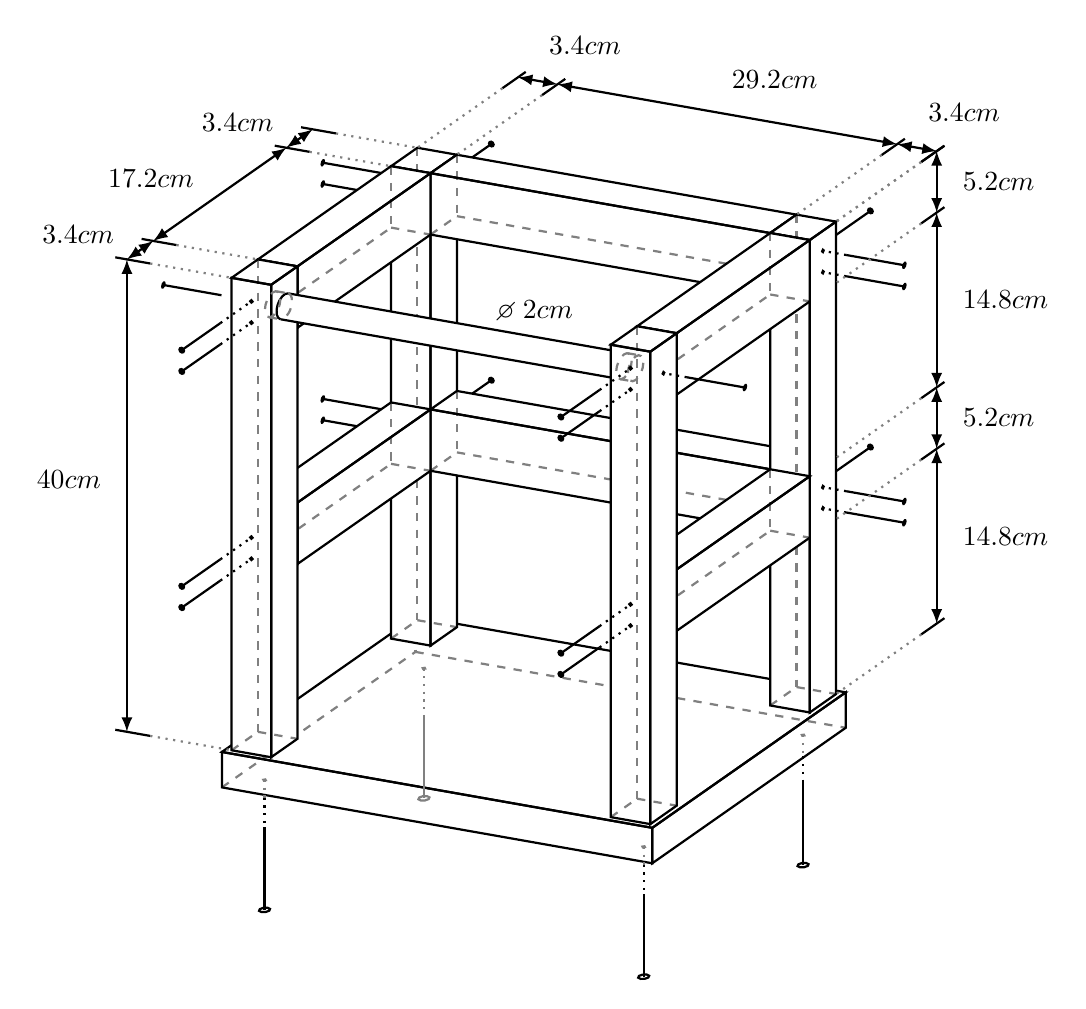
\begin{tikzpicture}

\newcommand{\rechteck}[6]
{
    \fill[white] (#1-#4/2,#2-#5/2,#3-#6/2) -- ++(#4,0,0) -- ++(0,0,#6) -- ++(0,#5,0) -- ++(-#4,0,0) -- ++(0,0,-#6) --cycle;
    % \fill[white] (#1-#4/2,#2-#5/2,#3-#6/2) -- ++(0,0,#6) -- ++(0,#5,0) -- ++(0,0,-#6) -- cycle;
    % \fill[white] (#1-#4/2,#2-#5/2,#3+#6/2) -- ++(#4,0,0) -- ++(0,#5,0) -- ++(-#4,0,0) -- cycle;

    \draw[dashed,gray] (#1+#4/2,#2-#5/2,#3-#6/2) -- ++(0,#5,0);
    \draw[dashed,gray] (#1-#4/2,#2+#5/2,#3-#6/2) -- ++(#4,0,0);
    \draw[dashed,gray] (#1+#4/2,#2+#5/2,#3-#6/2) -- ++(0,0,#6);

    \draw (#1-#4/2,#2-#5/2,#3-#6/2) -- ++(#4,0,0) -- ++(0,0,#6) -- ++(-#4,0,0) -- cycle;
    \draw (#1-#4/2,#2-#5/2,#3-#6/2) -- ++(0,0,#6) -- ++(0,#5,0) -- ++(0,0,-#6) -- cycle;
    \draw (#1-#4/2,#2-#5/2,#3+#6/2) -- ++(#4,0,0) -- ++(0,#5,0) -- ++(-#4,0,0) -- cycle;
}

% \begin{scope}[x={(.21cm,.15cm)},z={(.29cm,-.12cm)},y={(0cm,-.3cm)}]
\begin{scope}[x={(35:.12cm)},y={(90:-.15cm)},z={(-10:.15cm)}]
\path (1,0,0);
\pgfgetlastxy{\cylxx}{\cylxy}
\path (0,1,0);
\pgfgetlastxy{\cylyx}{\cylyy}
\path (0,0,1);
\pgfgetlastxy{\cylzx}{\cylzy}
\pgfmathsetmacro{\cylt}{(\cylzy * \cylyx - \cylzx * \cylyy)/ (\cylzy * \cylxx - \cylzx * \cylxy)}
\pgfmathsetmacro{\ang}{atan(\cylt)}
\pgfmathsetmacro{\ct}{1/sqrt(1 + (\cylt)^2)}
\pgfmathsetmacro{\st}{\cylt * \ct}

\begin{scope}[every path/.style={ thick}]
% \coordinate (0,0,0)

% schrauben vorne links
\foreach \y in {1.7,3.5,21.7,23.5} {
    \fill[black] (22.3,\y,-17) circle[radius=0.3];
    \draw (22.3,\y,-12) -- ++(0,0,-5);
}

% schrauben vorne
\foreach \y in{2.6,22.6} {
    \begin{scope}[canvas is zy plane at x=31, transform shape]
        \fill[black] (-8.3,\y) circle[radius=0.3];
        \fill[black] (24.3,\y) circle[radius=0.3];
    \end{scope}
    \draw (31,\y,-8.3) -- ++(-5,0,0);
    \draw (31,\y,24.3) -- ++(-5,0,0);
}

% schrauben hinten links
\fill[black] (1.7,2.6,-17) circle[radius=0.3];
\draw (1.7,2.6,-12) -- ++(0,0,-5);

\rechteck{12}{41.5}{8}{25}{3}{37};

% pfosten vorne links
\rechteck{22.3}{20}{-8.3}{3.4}{40}{3.4};

% sprossen vorne
\rechteck{22.3}{2.6}{8}{3.4}{5.2}{29.2};
\rechteck{22.3}{22.6}{8}{3.4}{5.2}{29.2};

% sprossen links
\rechteck{12}{2.6}{-8.3}{17.2}{5.2}{3.4}
\rechteck{12}{22.6}{-8.3}{17.2}{5.2}{3.4}

% pfosten hinten links
\rechteck{1.7}{20}{-8.3}{3.4}{40}{3.4};

% pfosten vorne rechts
\rechteck{22.3}{20}{24.3}{3.4}{40}{3.4};

% sprossen rechts
\rechteck{12}{2.6}{24.3}{17.2}{5.2}{3.4}
\rechteck{12}{22.6}{24.3}{17.2}{5.2}{3.4}

% stange
\fill[white] (\ct+1.7,\st+2.6,-6.6) -- ++(0,0,29.2) arc[start angle=\ang,delta angle=180,radius=1] -- ++(0,0,-29.2) arc[start angle=\ang+180,delta angle=180,radius=1];
\draw (\ct+1.7,\st+2.6,-6.6) -- ++(0,0,29.2);
\draw (-\ct+1.7,-\st+2.6,-6.6) -- ++(0,0,29.2);

% pfosten hinten rechts
\rechteck{1.7}{20}{24.3}{3.4}{40}{3.4};

%stangenloch rechts
\draw[dashed,gray] (1.7,2.6,23.6) circle[radius=1];
\draw[dashed,gray] (1.7,2.6,22.6) circle[radius=1];
\draw[dashed,gray] (\ct+1.7,\st+2.6,22.6) -- ++(0,0,1);
\draw[dashed,gray] (-\ct+1.7,-\st+2.6,22.6) -- ++(0,0,1);

% stange
\draw[dashed,gray] (\ct+1.7,\st+2.6,-6.6) arc[start angle=\ang,delta angle=180,radius=1];
\draw (\ct+1.7,\st+2.6,-6.6) arc[start angle=\ang,delta angle=-180,radius=1];

%stangenloch rechts
\draw[dashed,gray] (1.7,2.6,-7.6) circle[radius=1];
\draw[dashed,gray] (\ct+1.7,\st+2.6,-7.6) -- ++(0,0,1);
\draw[dashed,gray] (-\ct+1.7,-\st+2.6,-7.6) -- ++(0,0,1);

% schrauben richts hinten
\fill[black] (1.7,2.6,33) circle[radius=0.3];
\draw (1.7,2.6,33) -- ++(0,0,-5);
\draw (1.7,2.6,26) circle[radius=0.1];
\draw[dotted] (1.7,2.6,28) -- ++(0,0,-2);

\

% schrauben hinten und rechts vonre
\foreach \z in {1.7,3.5,21.7,23.5} {
    % rechts vorne
    \fill[black] (22.3,\z,33) circle[radius=0.3];
    \draw (22.3,\z,33) -- ++(0,0,-5);
    \draw (22.3,\z,26) circle[radius=0.1];
    \draw[dotted] (22.3,\z,28) -- ++(0,0,-2);
    % hinten
    \begin{scope}[canvas is zy plane at x=-9, transform shape]
        \fill[black] (-8.3,\z) circle[radius=0.3];
        \fill[black] (24.3,\z) circle[radius=0.3];
    \end{scope}
    \draw (-9,\z,-8.3) -- ++(5,0,0);
    \draw (-9,\z,24.3) -- ++(5,0,0);
    \begin{scope}[canvas is zy plane at x=0, transform shape]
        \draw (-8.3,\z) circle[radius=0.1];
        \draw (24.3,\z) circle[radius=0.1];
    \end{scope}
    \draw[dotted] (-4,\z,-8.3) -- ++(4,0,0);
    \draw[dotted] (-4,\z,24.3) -- ++(4,0,0);
}

% schrauben unten
% \rechteck{12}{41.5}{8}{25}{3}{37};
% schrauben
\draw (1.7,47,-8.3) -- ++(0,7,0);
\draw (1.7,47,24.3) -- ++(0,7,0);
\draw[gray] (22.3,47,-8.3) -- ++(0,7,0);
\draw (22.3,47,24.3) -- ++(0,7,0);
% sichtbare dotts
\draw[dotted] (1.7,44.5,-8.3) -- ++(0,2.5,0);
\draw[dotted] (1.7,44.5,24.3) -- ++(0,2.5,0);
\draw[dotted] (22.3,44.8,24.3) -- ++(0,2.2,0);
% verdeckte dotts
\draw[dotted,gray] (22.3,43,-8.3) -- ++(0,4,0);
\draw[dotted,gray] (1.7,43,-8.3) -- ++(0,1.5,0);
\draw[dotted,gray] (1.7,43,24.3) -- ++(0,1.5,0);
\draw[dotted,gray] (22.3,43,24.3) -- ++(0,1.5,0);
%schraubenköpfe
\begin{scope}[canvas is xz plane at y=54, transform shape]
    \draw (1.7,-8.3) circle[radius=0.4];
    \draw (1.7,24.3) circle[radius=0.4];
    \draw[gray] (22.3,-8.3) circle[radius=0.4];
    \draw (22.3,24.3) circle[radius=0.4];
\end{scope}
% bohrmarker
\begin{scope}[canvas is xz plane at y=43, transform shape]
    \draw[gray] (1.7,-8.3) circle[radius=0.1];
    \draw[gray] (1.7,24.3) circle[radius=0.1];
    \draw[gray] (22.3,-8.3) circle[radius=0.1];
    \draw[gray] (22.3,24.3) circle[radius=0.1];
\end{scope}
% maße

\tikzstyle{dim}    = [latex-latex]

\foreach \x in {0,3.4,20.6,24} {
    \draw (\x,0,-20) -- ++ (0,0,3);
    \draw[dotted,gray] (\x,0,-17) -- (\x,0,-10);
}
\foreach \x/\label in {0/3.4,3.4/17.2,20.6/3.4} {
    \draw[dim] (\x,0,-19) -- ++ (\label,0,0) node[midway,left,yshift=0.2cm,xshift=-0.2cm] {\label$ cm$};
}

\draw (0,40,-20) -- ++ (0,0,3);
\draw[dotted,gray] (0,40,-17) -- (0,40,-10);
\draw[dim] (0,0,-19) -- ++ (0,40,0) node[midway,left,yshift=0.2cm,xshift=-0.2cm] {40$ cm$};


\foreach \z in {-10,-6.6,22.6,26} {
    \draw (35,0,\z) -- ++ (3,0,0);
    \draw[dotted,gray] (35,0,\z) -- (24,0,\z);
}
\foreach \z/\label in {-10/3.4,-6.6/29.2,22.6/3.4} {
    \draw[dim] (37,0,\z) -- ++ (0,0,\label) node[midway,above,yshift=0.2cm,xshift=0.6cm] {\label$ cm$};
}

\foreach \y in {0,5.2,20,25.2,40} {
    \draw (35,\y,26) -- ++ (3,0,0);
    \draw[dotted,gray] (35,\y,26) -- (24,\y,26);
}
\foreach \y/\label in {0.0/5.2,5.2/14.8,20/5.2,25.2/14.8} {
    \draw[dim] (37,\y,26) -- ++(0,\label,0) node[midway,right,xshift=0.2cm] {\label$ cm$};
}

\path (0,0,16) node[above] {$\diameter \: 2cm$};


% \draw (0,0,0) circle[radius=1];
% \draw[->] (0,0,0) -- (1,0,0);
% \draw[->] (0,0,0) -- (0,1,0);
\end{scope}
\end{scope}

\end{tikzpicture}
\end{document}
